\documentclass[aspectratio=169]{beamer}
\usepackage{goethecc}

\usepackage{color, colortbl}

\usepackage[USenglish]{babel}
\usepackage{amsmath,amsfonts,amssymb,textcomp}
\usepackage{graphicx}
\usepackage{pdfpages}


\usepackage{latexsym}
\usepackage{xspace}

\usepackage{aurical}

\usepackage{intcalc}

\usepackage{siunitx}
%%%%%%%%%%%% Turing Machine State Diagram
\def\tmKeyBasename#1#2.#3\relax{\xdef#1{#2}}

\newcommand{\tmDrawStates}[1]{
	% set \tmHeadChar
	\tmCurrentChar
	
	
    \def\tmstate##1##2##3##4{
        % 1 key
        % 2 label
        % tikz options
        % tikz position

        \node[
            tm-state,
            onif={<\equal{##1}{\tmStateCurrent}>tm-state-active},
            ##3
        ] (##1) ##4 {##2};
    }

    \def\tmstart##1{
        \path[tm-trans]  ($(##1.west)-(1.5em, 0)$) to ++(1.5em, 0);
    }

    \def\tmtrans##1##2##3##4##5{{
        % 1 current state
        % 2 next state
        % 3 instruction
        % 4 format path
        % 5 format label

		% Disable the newline comannd (only for this scope, though)
		\renewcommand{\\}{}
		
		\tmKeyBasename\tmDrawSourceBase##1.\relax		
		\tmKeyBasename\tmDrawTargetBase##2.\relax		

		% First find out if this is an active edge
        \def\tmDrawTransActiveEdge{}
        {
			% Parameter ##3 contains a list of \trans commands;
			% that's all we are interested in. Gather the infos
			% via the local version of \trans!
		    \def\trans####1####2####3{%
	    		\ifthenelse{\equal{\tmStateCurrent}{\tmDrawSourceBase} \AND \equal{\tmHeadChar}{####1}}{%
	    			\gdef\tmDrawTransActiveEdge{tm-trans-active}%
	    		}{}%
		    }%
			##3
        }
        
		% Build the label and store it in the following macro        
        \def\tmDrawTransLabel{}
	    {
	        % Parameter ##3 contains a list of \trans commands;
			% that's all we are interested in. Gather the infos
			% via the local version of \trans!
            \def\trans####1####2####3{%
            	% Human readable direction
            	\ifthenelse{\equal{####3}{L}}{%
            		\def\tmDrawTransDir{$\Leftarrow$}%
            	}{\ifthenelse{\equal{####3}{R}}{%
            		\def\tmDrawTransDir{$\Rightarrow$}%
            	}{%
	            	\def\tmDrawTransDir{$\Downarrow$}%
	            }}%

				% Make active transition label red, remainder black
				\ifthenelse{\equal{\tmStateCurrent}{\tmDrawSourceBase} \AND \equal{\tmHeadChar}{####1}}{
					\edef\transLabelColor{emorot}
				}{
					\edef\transLabelColor{black}
				}

				% Short-Cut             	
            	\def\transLabel{%
            		\noexpand\textcolor{\transLabelColor}{%
	            		\noexpand\texttt{####1} zu \noexpand\texttt{####2}, \tmDrawTransDir%
	            	}%
            	}%

				\xdef\tmDrawTransLabel{
					\unexpanded\expandafter{\tmDrawTransLabel}%
					\tmDrawTransLabelNewLine % Empty in first iteration, otherwise \\
					\transLabel
		    	}%
		    	
			    % Seperate several transition with newline
		    	\def\tmDrawTransLabelNewLine{\noexpand\\}
            }%

	        \def\tmDrawTransLabelNewLine{}
            ##3
        }
        

        \path[tm-trans, \tmDrawTransActiveEdge, ##4] 
	        (##1) to 	% source
	        node[align=center, ##5] {\tmDrawTransLabel} % label
	        (##2) % target
	    ;
    }}

	\begin{tikzpicture}[
		node distance = 4em and 15em,
		on grid,
		tm-state/.style={draw, minimum width=6em},
		tm-state-active/.style={fill=emorot!50},
		tm-state-next/.style={blue},
		tm-trans/.style={draw, ->, shorten >=2pt, thick, auto},
		tm-trans-active/.style={emorot},
		loop above/.style={looseness=8, out=120, in=60},
		loop below/.style={looseness=8, out=300, in=240}
	]
		#1
    \end{tikzpicture}
}



%%%%%%%%%%%% Turing Machine Band Diagram and Band Helpers
\def\tmCurrentCharHelp#1@#2@#3\relax{\xdef\tmHeadChar{#2}}%
\newcommand{\tmCurrentChar}{\expandafter\tmCurrentCharHelp\tmBand\relax}


\newcounter{tmBandCnt}
\newcounter{tmBandCntHead}

\newcommand{\tmDrawBand}{
	\def\decreasedCounter##1{\numexpr\value{##1} - 1\relax}
	
	\def\tmbandCellCaption##1{%
		\ifthenelse{\equal{##1}{B}}{$\mathbb B$}{##1}%
	}	
	
	\def\turingBandHelp##1##2##3##4\relax{%
		\ifx##1\relax{}\else{%
			\stepcounter{tmBandCnt}
			\ifthenelse{\equal{##1}{@}}{%
				\node[tmCellActive, onif={<\equal{##2}{B}>tmCellBlank}] (tmbandcell\thetmBandCnt) at ($(tmbandcell0) + (\thetmBandCnt*\cellSize,0)$) {\tmbandCellCaption##2};
				\setcounter{tmBandCntHead}{\thetmBandCnt}%
				\turingBandHelp##4\relax\relax\relax\relax%		
			}{%
				\node[tmCell, onif={<\equal{##1}{B}>tmCellBlank}] (tmbandcell\thetmBandCnt) at ($(tmbandcell0) + (\thetmBandCnt*\cellSize,0)$) {\tmbandCellCaption##1};
				\turingBandHelp##2##3##4\relax\relax\relax%
		}%
	}
	\fi%
	}
	
	
	
	\begin{tikzpicture}[remember picture]
		\node[tmCell] (tmbandcell0) {};
	
		\setcounter{tmBandCnt}{0}
		\setcounter{tmBandCnt}{0}
		\expandafter\turingBandHelp\tmBand\relax\relax\relax\relax
	
		\ifthenelse{\equal{\thetmBandCntHead}{0}}{}{
			\node[tmHeadMarker, at=(tmbandcell\thetmBandCntHead)] (tmheadmarker) {};				
		}
	\end{tikzpicture}
}

\newcommand{\tmDrawGrid}[2]{
	\foreach \i in {#1, ..., #2} {
		\path[draw] ($(tmbandcell0.north west)+(\i*\cellSize, 0)$) 
		to ($(tmbandcell0.south west)+(\i*\cellSize, 0)$);
	}
	
	\path[draw] ($(tmbandcell0.north west)+(#1*\cellSize, 0)$) 
	to ($(tmbandcell0.north west)+(#2*\cellSize, 0)$);
	
	\path[draw] ($(tmbandcell0.south west)+(#1*\cellSize, 0)$) 
	to ($(tmbandcell0.south west)+(#2*\cellSize, 0)$);
}




%%%%%%%%%%%% Turing Machine Execution
\def\tmMoveLeftHelp#1#2#3#4#5\relax{{%
	\ifx#1@%
		% Move left before start: Insert Blank Symbol
		\xdef\tmNewBand{@B@#2#4#5}%
	\else%
		\ifx#4\relax%
			% This is not possible in an input containing @
			ILLEGAL INPUT%
		\else
			\ifx#2@%
				\xdef\tmNewBand{\tmNewBand @#1@#3#5}%
			\else%
				\xdef\tmNewBand{\tmNewBand#1}%
				\tmMoveLeftHelp#2#3#4#5\relax\relax%
			\fi%
		\fi%
	\fi
}}

\def\tmMoveRightHelp#1@#2@#3#4\relax{{%
	\ifx#3\relax
		\xdef\tmNewBand{#1#2@B@}%
	\else
		\xdef\tmNewBand{#1#2@#3@#4}%
	\fi
}}

\newcommand{\tmMoveLeft}{%
	\def\tmNewBand{}%
	\expandafter\tmMoveLeftHelp\tmBand\relax\relax\relax\relax\relax%
	\xdef\tmBand{\tmNewBand}
}

\newcommand{\tmMoveRight}{%
	\def\tmNewBand{}%
	\expandafter\tmMoveRightHelp\tmBand\relax\relax\relax\relax\relax%
	\xdef\tmBand{\tmNewBand}
}




\def\tmWriteCharHelp#1@#2@#3\relax{\xdef\tmBand{#1@\tmCharToWrite@#3}}%
\newcommand{\tmWriteChar}[1]{%
	\def\tmCharToWrite{#1}%
	\expandafter\tmWriteCharHelp\tmBand\relax%
}

\def\tmExecTrans#1#2#3#4#5\relax{
	\if\tmHeadChar#1
		\tmWriteChar#2
		\if#3L
			\tmMoveLeft
		\else\if#3R
			\tmMoveRight
		\fi\fi
		\csname#4\endcsname
	\else
		\if\relax\detokenize{#5}\relax\else
			\tmExecTrans#5\relax
		\fi
	\fi
}

\def\tmShowBandHelp#1@#2@#3\relax{%
	\texttt{#1\underline{#2}#3}%
}

\newcommand{\tmShowBand}{
	\expandafter\tmShowBandHelp\tmBand\relax	
}


%%%%%%%%%%%%% TM Parser
\newcommand{\tmSetup}[2]{{
	% This macro will interpret a TM specification 
	% as defined the three operations:
	%  \tmstate{X}{}{}{} where X is the state's key
	%  \tmstart{X} where X is the start state's key
	%  \tmtrans{X}{Y}{Z}{}{} where 
	%     X is the source state's key
	%     Y is the target state's key
	%     Z is a transition list consisting of 
	%     \trans{A}{B}{C} commands where
	%		A is the read character
	%       B the replacement
	%       C the movement {L, R, H}
	
	% The setup process creates a number of macrocs
	% with a tmImpl#1 prefix. Each state X gets two
	% macros tmImpl#1TransX which contains a list of
	% transitions (each transition is defined by 
	% exactly four tokens) and tmImpl#1X which is
	% "callable" transition.
		
	\def\tmCurrentName{#1}
	
	\newcommand{\tmstate}[4]{%
		\expandafter\xdef\csname tmImpl\tmCurrentName Trans##1\endcsname{}
		\expandafter\xdef\csname tmImpl\tmCurrentName ##1\endcsname{}
	}
	
	\newcommand{\tmstart}[1]{
		\expandafter\xdef\csname tmImpl\tmCurrentName Start\endcsname{##1}
	}

	\newcommand{\trans}[3]{
		\xdef\tmTransAccum{\tmTransAccum##1##2##3{\tmTransTargetKey}}
	}
	\newcommand{\tmtrans}[5]{
		\tmKeyBasename\tmImplSourceBase##1.\relax		
		\tmKeyBasename\tmImplTargetBase##2.\relax
		
		\xdef\tmTransTargetKey{tmImpl\tmCurrentName\tmImplTargetBase}
		\def\tmTransAccum{}
		
		
		##3
		
		\expandafter\xdef\csname tmImpl\tmCurrentName Trans\tmImplSourceBase\endcsname{%
			\csname tmImpl\tmCurrentName Trans\tmImplSourceBase\endcsname%
			\tmTransAccum
		}

		\expandafter\xdef\csname tmImpl\tmCurrentName\tmImplSourceBase\endcsname{%
			\noexpand\tmCurrentChar%
			\noexpand\csname tmImpl\tmCurrentName StateCallback\endcsname{\tmImplSourceBase}%
			\noexpand\tmExecTrans\csname tmImpl\tmCurrentName Trans\tmImplSourceBase\endcsname\noexpand\relax
		}
	}

	% tmTrans Definitions may include newlines; redefine command to prevent output
	\renewcommand{\\}{}	
	#2
}}


\def\tmSetInitialBand#1#2\relax{\xdef\tmBand{@#1@#2}}
\newcommand{\tmExecute}[3]{
	\tmSetInitialBand#2\relax
	\expandafter\gdef\csname tmImpl#1StateCallback\endcsname{#3}
	\csname tmImpl#1\csname tmImpl#1Start\endcsname\endcsname
}


\sisetup{locale = DE}

\usepackage{xstring}
\usepackage{tikz}
\usepackage{pgf}
\usepackage{mathtools,pgfplots}
\usetikzlibrary{calc}   
\usetikzlibrary{positioning}
\usetikzlibrary{automata}
\usetikzlibrary{arrows}   
\usetikzlibrary{backgrounds}

\usepackage{soul}
\graphicspath{{./images/}}
\usepackage{listings}
\usepackage{qrcode}


%%%%%%%%%%%%%%%%%%%%%%%%%%%%%%%%%%%%%%%%%%%%
% We gonna write a lot of unary numbers; let TeX do the work for us
\newcommand{\unum}[1]{
	\ifthenelse{\equal{0}{#1}}{}{
	\ifthenelse{\equal{1}{#1}}{1}{%
	1%
	\foreach \unumj in {\intcalcDec{#1},...,1} {%
		\ifthenelse{\equal{\intcalcMod{\unumj}{3}}{0}}{\textquoteleft}{}%<-- this is the sep
		1%<-- this is the actual digit
	}%
}}}
\newcommand{\ttunum}[1]{\ensuremath{\mathtt{\unum{#1}}}}


%%%%%%%%%%%%%%%%%%%%%%%%%%%%%%%%%%%%%%%%%%%%
% General purpose tikz attributes for condition formating
\tikzset{onslide/.code args={<#1>#2}{%
    \only<#1>{\pgfkeysalso{#2}} % \pgfkeysalso doesn't change the path
}}
\tikzset{onslidep/.code args={<#1>#2}{%
		\ifthenelse{#1 = 0}{}{\only<#1->{\pgfkeysalso{#2}}} % \pgfkeysalso doesn't change the path
}}
\tikzset{onslidepp/.code args={<#1><#2>#3}{%
		\ifthenelse{#1=0 \OR #2=0}{}{\only<#1-#2>{\pgfkeysalso{#3}}} % \pgfkeysalso doesn't change the path
	}}
\tikzset{temporal/.code args={<#1>#2#3#4}{%
    \temporal<#1>{\pgfkeysalso{#2}}{\pgfkeysalso{#3}}{\pgfkeysalso{#4}} % \pgfkeysalso doesn't change the path
}}
\tikzset{onif/.code args={<#1>#2}{%
 	\ifthenelse{#1}{\pgfkeysalso{#2}}{}%
}}

\newcommand{\tikzanchor}[1]{\tikz[overlay, remember picture]{\node[anchor=text, inner sep=0] (#1) {\phantom{Ig}};}}
\newcommand{\tikzanchortext}[2]{\tikz[overlay, remember picture]{\node[anchor=text, inner sep=0] (#1) {#2};}}


%%%%%%%%%%%%%%%%%%%%%%%%%%%%%%%%%%%%%%%%%%%%
% Formating of our Turing Machines 		
\def\cellSize{27pt}
\def\tmBlankSym{\ensuremath{\mathbb B}}
		
\tikzset{tmCell/.style={font={\Large\tt}, minimum height=\cellSize, minimum width=\cellSize}}
\tikzset{tmCellActive/.style={tmCell}}
\tikzset{tmCellBlank/.style={dunkelgrau!50, fill=sandgrau}}
\tikzset{tmHeadMarker/.style={circle, draw, ultra thick, emorot, minimum width=0.9*\cellSize, minimum height=0.9*\cellSize}}

\tikzset{tmState/.style={draw, minimum width=6em, rounded corners=0.4em}}
\tikzset{tmStateActive/.style={fill=emorot!50}}
\tikzset{tmTrans/.style={draw, ->, shorten >=2pt, thick, auto}}
\tikzset{tmTransActive/.style={emorot}}


\tikzset{loop above/.style={looseness=8, out=120, in=60}}
\tikzset{loop below/.style={looseness=8, out=300, in=240}}
\pgfplotsset{compat=1.13}

\lstset{
	language=[LaTeX]{TeX},
	basicstyle=\small\sffamily,
	numbers=left,
	numberstyle=\tiny,
	commentstyle=\color{goetheblau},
	frame=tb,
	columns=fullflexible,
	showstringspaces=false,
	morekeywords={\tmstate, \tmstart, \tmtrans, \trans},
	escapechar={\$},
	xleftmargin=2em
}


\begin{document}
\title{
	Und womit rechnest du so? \\[-0.5em]
	\textcolor{dunkelgrau}{\small \emph{mit Folien von Cyriax und Manuel}}
}
\author{
	Jonathan Cyriax Brast\\
	Manuel Penschuck \\
} 
\date{10. Juni 2017}

{
\setbeamertemplate{footline}{} 
\goethccBgTitel
\begin{frame}
  \titlepage
  \begin{tikzpicture}[overlay]
	  \node[anchor=south east, xshift=-0.08\textwidth, yshift=0.05\textheight, at=(current page.south east)] {
\includegraphics[width=0.15\textwidth]{cs.pdf}};
  \end{tikzpicture}
\end{frame}
}
\addtocounter{framenumber}{-1}


%\frame{\frametitle{Outline}\tableofcontents}

%%%%%%%%%%%%%

\begin{frame}{}
	\begin{center}
		\scalebox{1.5}{\Huge \textcolor{emorot}{Subtraktion}}
		
		\vspace{1em}
		
		{\large \textcolor{goetheblau}{Minus-Rechnen}}
	\end{center}
\end{frame}


\begin{frame}{Subtraktion}
	\begin{center}
		\Huge

		\only<+>{
			\scalebox{1.5}{\Huge \textcolor{emorot}{Selbsttest}}
		}		
		\only<+>{$\textcolor{goetheblau}{7}-\textcolor{emorot}{3}=\underline{\phantom4}$}
		\only<+>{$\textcolor{goetheblau}{7}-\textcolor{emorot}{3}=\textcolor{orange}{\underline{4}}$}
		
		\only<+>{
			\scalebox{1.5}{\Huge \textcolor{emorot}{Und noch einer \ldots}}
		}		
		\only<+>{$\textcolor{goetheblau}{123}-\textcolor{emorot}{45}=\underline{\phantom{78}}$}
		\only<+>{
			$\textcolor{goetheblau}{123}-\textcolor{emorot}{45}=\textcolor{orange}{\underline{78}}$
			\begin{tikzpicture}[overlay, remember picture]
				\node[at=(current page.south east), anchor=south east, xshift=-2em, yshift=2em]  {\Large \color{sandgrau} \#NotMyPisa};
			\end{tikzpicture}
		}
	\end{center}
\end{frame}

\begin{frame}{Unäre Zahlen -- römisch für Arme}
	\begin{tikzpicture}[remember picture, overlay]
	\node[at=(current page.north), yshift=-3em, anchor=north, draw, fill=sandgrau, minimum width=2\textwidth, minimum height=2.5em] {
		\large
		Wir stellen die \textcolor{goetheblau}{Zahl $x$} durch  \textcolor{emorot}{$x$ Einsen} dar.
	};
	\end{tikzpicture}


	\begin{center}
		\begin{tikzpicture}[
			node distance=0,
			dnum/.style={align=right, text width=2em},
			unum/.style={align=right, text width=8em}
		]
			\node (a0) {};
			\foreach \i in {1, ..., 5} {
				\node[dnum, below=of a\intcalcDec\i] (a\i) {$\textcolor{goetheblau}{\i}_\text{Dez}$};
				\node[right=of a\i] (b\i) {$=$};
				\node[unum, right=of b\i] (c\i) {$\textcolor{emorot}{\ttunum{\i}}_\text{Unär}$};
	
				\node[dnum, right=2em of c\i] (d\i) {$\textcolor{goetheblau}{\intcalcAdd5\i}_\text{Dez}$};
				\node[right=of d\i] (e\i) {$=$};
				\node[unum, right=of e\i] (f\i) {$\textcolor{emorot}{\ttunum{\intcalcAdd5\i}}_\text{Unär}$};
			}
		\end{tikzpicture}
	\end{center}
\end{frame}

\begin{frame}{Wie beschreiben wir unäre Subtraktion?}
	\vspace{4.5em}

	\begin{center}
		\scalebox{1.3}{
			\begin{tikzpicture}[
				number/.style={text width=3.8em, align=right, anchor=north west, inner sep=0.1em, minimum height=1.5em, orange},
				header/.style={number, font={\bf}}
			]
				\def\sx{4em}
				\def\sy{1.5em}
	
				\node[fill=sandgrau, anchor=north west, minimum width=7*\sx, minimum height=\sy, inner sep=0] at (0,0)  {};
				\node[fill=sandgrau, anchor=north west, minimum width=\sx, minimum height=11em, inner sep=0] at (0,0)  {};
			
				\foreach \x in {1, ..., 5} {
					\node[header, goetheblau] at (\x*\sx, 0) {$\mathbf{\unum{\x}}$};
					\node[header, emorot] at (0, -\x*\sy) {$\mathbf{\unum{\x}}$};
	
					\node[header, goetheblau] at (6*\sx, 0) {$\cdots$};
					\node[header, emorot, minimum height=2em] at (0, -6*\sy) {$\vdots$\ \ \phantom.};
	
					\node[number, fill=sandgrau] at (6*\sx, -\x*\sy) {$\cdots$};
					\node[number, fill=sandgrau, minimum height=2em] at (\x*\sx, -6*\sy) {$\vdots$};
	
					
					\foreach \y in {1, ..., 5} {
						\ifthenelse{\equal{\intcalcCmp\x\y}{-1}}{
							\node[number, fill=sandgrau] at (\x*\sx, -\y*\sy) {};
						}{
							\node[number] at (\x*\sx, -\y*\sy) {
								\ifthenelse{\equal\x\y}{\textcolor{emorot}{\only<2>{0}}} 
								{\ttunum{\intcalcSub\x\y}}
							};
						}
					}
				}
				
				\node[header, fill=sandgrau, minimum height=2em] at (6*\sx, -6*\sy) {$\ddots$};
				
				\node[goetheblau, draw, minimum width=28em, minimum height=11em, anchor=north west, onslide={<4->white, fill=white, opacity=0.8}] (tabborder) {};
			\end{tikzpicture}
		}
	\end{center}

	\begin{tikzpicture}[remember picture, overlay]
		\node[at=(current page.north), yshift=-3em, anchor=north, draw, fill=sandgrau, minimum width=2\textwidth, minimum height=2.5em] {
			\Huge
			$\textcolor{goetheblau}{a} - \textcolor{emorot}{b} = \textcolor{orange}{c}$
		};
		
		\only<4->{
			\node[draw, radius=0.5em, rounded corners=1em, emorot, fill=white, opacity=0.8, inner sep=2em] at (current page) {\phantom{\Huge Nicht praktikabel für große Zahlen!}};
			
			\node[emorot, inner sep=2em] at (current page) {\Huge Unpraktisch für große Zahlen!};
		}
	\end{tikzpicture}
\end{frame}

\newcommand{\removeDigit}[1]{%
	\only<-\intcalcDec{#1}>{1}%
	\only<#1>{\textcolor{emorot}{\underline 1}}%
}

\begin{frame}{Wir brauchen einen Algorithmus}
	\begin{tikzpicture}[remember picture, overlay]
	\node[at=(current page.north), yshift=-3em, anchor=north, draw, fill=sandgrau, minimum width=2\textwidth] {
		\Huge
		$\textcolor{goetheblau}{a} - \textcolor{emorot}{b} = \textcolor{orange}{c}$
	};
	\end{tikzpicture}
	
	\begin{columns}[t]
		\begin{column}{0.7\textwidth}
			\Large
			\setbeamertemplate{enumerate items}[default]
			\begin{enumerate}
				\item
					\tikzanchor{step1}%
					\textbf{Wenn} \textcolor{emorot}{$b$} keine Ziffer mehr hat,\\
					\tikzanchor{step1a}
					\textbf{dann} \textcolor{orange}{\textbf{antworte} $c \gets a$} und \textbf{halte}
					
					\vspace{1em}

				
				\item
					\tikzanchor{step2}%
					\texttt{Entferne} letzte Ziffer von \textcolor{goetheblau}{a}\\
					\texttt{Entferne} letzte eine Ziffer von \textcolor{emorot}{b}

					\vspace{1em}

				
				\item 
					\tikzanchor{step3}%
					\textbf{Springe} zu \textcolor{goetheblau}{1.}
			\end{enumerate}
		\end{column}%
		
		\begin{column}{0.25\textwidth}
			\Huge

			$\textcolor{goetheblau}{a}$: \hfill 1\removeDigit6\removeDigit3\\
			$\textcolor{emorot}{b}$: \hfill \removeDigit6\removeDigit3\\
			$\textcolor{orange}{c}$: \hfill \only<-8>{?}\only<9>{\textcolor{emorot}{1}}
			
			\uncover<9>{\begin{center}
					Halt, Stop!
			\end{center}}
			
		\end{column}
	\end{columns}
	
	\begin{tikzpicture}[
		overlay, remember picture,
		prog counter/.style={emorot, <-, ultra thick}
	]
		\path[prog counter, onslide={<2,5,8>draw}] ($(step1)+(-2.5em,0)$) to ++(-2em, 0);
		\path[prog counter, onslide={<9>draw}]     ($(step1a)+(-2.5em,0)$) to ++(-2em, 0);		
		\path[prog counter, onslide={<3,6>draw}]   ($(step2)+(-2.5em,0)$) to ++(-2em, 0);
		\path[prog counter, onslide={<4,7>draw}]   ($(step3)+(-2.5em,0)$) to ++(-2em, 0);
	
	\end{tikzpicture}
	
\end{frame}


\newcommand{\handwrittenNoteBelow}[3]{
	\node[goetheblau, anchor=west, align=left] at ($(#1)+(1.6,-0.6)#3$) {\Large \Fontauri\bfseries #2};
	\path[<-, draw, goetheblau, ultra thick, bend right=15] ($(#1)#3$) to ++(1.5,-0.5);
}

\newcommand{\handwrittenNoteAbove}[3]{
	\node[goetheblau, anchor=west, align=left] at ($(#1)+(1.6,0.6)#3$) {\Large \Fontauri\bfseries #2};
	\path[<-, draw, goetheblau, ultra thick, bend left=15] ($(#1)#3$) to ++(1.5,0.5);
}


\begin{frame}{}
	\begin{center}
		\Huge
		\only<1>{Turing Maschine}
		
		\large
		\only<2-3>{%
			\only<2>{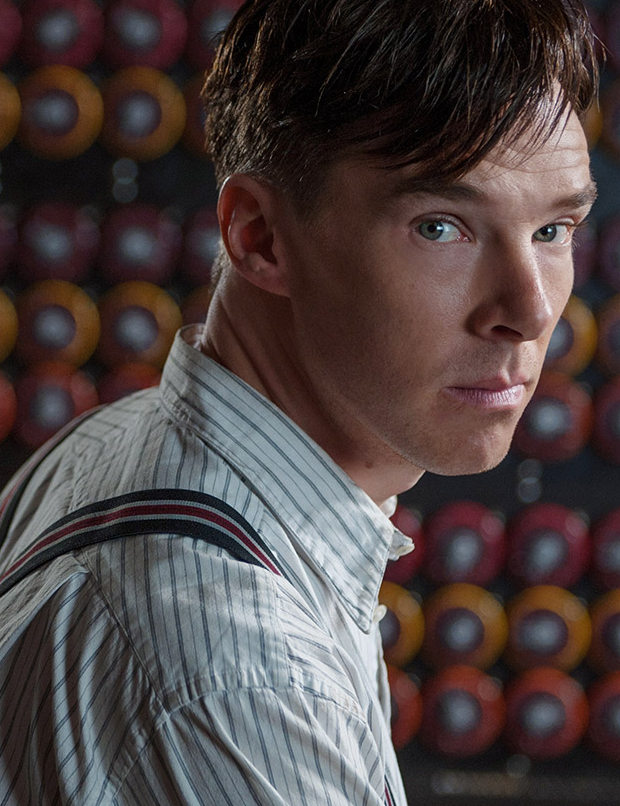
\includegraphics[height=0.6\textheight]{images/cumberbatch.jpg}}%
			\only<3>{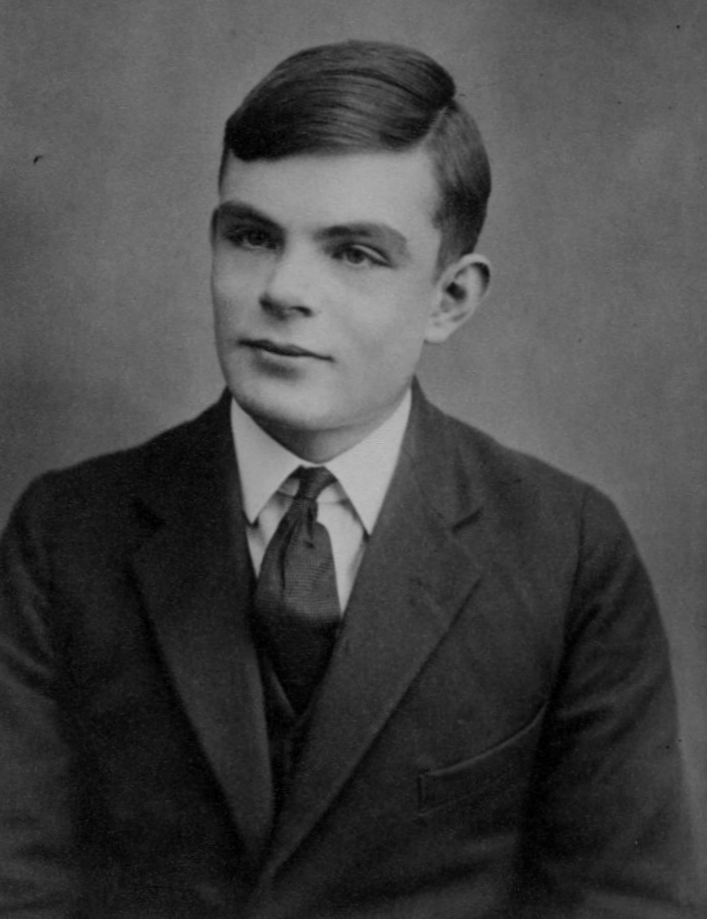
\includegraphics[height=0.6\textheight]{images/turing.jpg}}%
			\hspace{2em}
			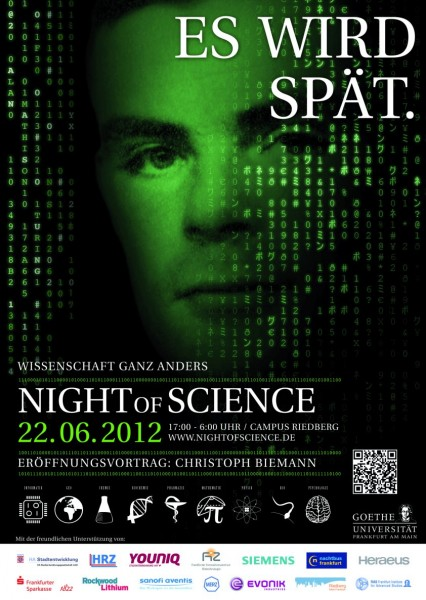
\includegraphics[height=0.6\textheight]{images/nos2012.jpg}
			\vspace{1em}
						
			Alan M. Turing\\
			1912 -- 1954 
		}
		\only<4>{
			\fbox{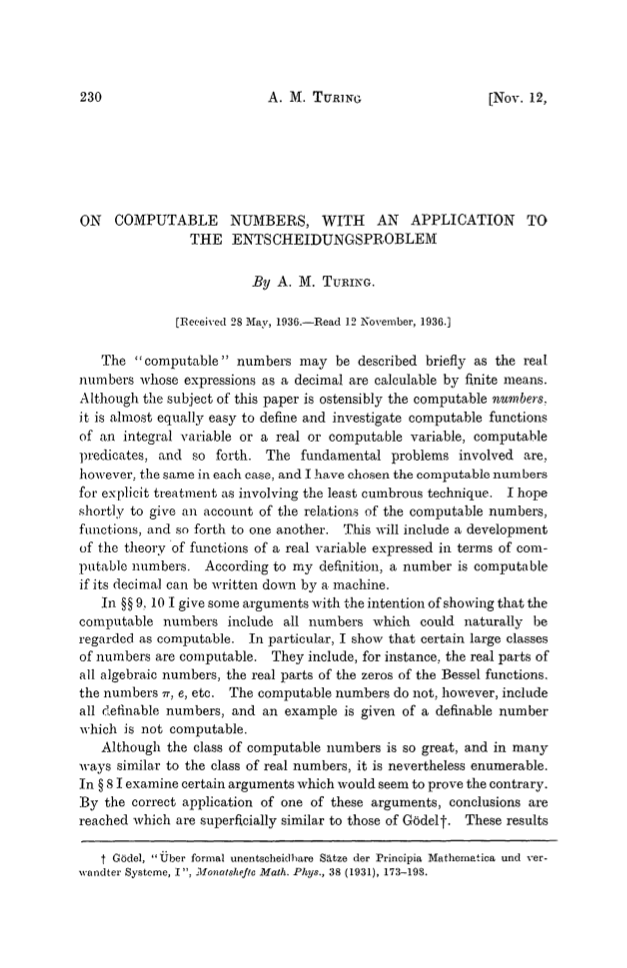
\includegraphics[height=0.6\textheight]{images/turing1936.png}}
			\vspace{1em}
			
			\textquotedblleft On Computable Numbers, With an Application to the Entscheidungsproblem\textquotedblright\\
			\textcolor{goetheblau}{[A. Turing, 1936/37]}
		}
	\end{center}
\end{frame}


\begin{frame}{Turing Maschine}
	\begin{center}
		\vspace{2em}

		\uncover<7->{
			\begin{tikzpicture}[remember picture]
				\node[tmState, draw] (stateA) {Zustand A};
				\node[tmState, draw, anchor=west] (stateB) at ($(stateA.east) + (5,0)$)  {Zustand B};
				
				\path[draw, ->, thick, bend left=10, shorten >=5pt, onslide={<8>, emorot}] (stateA) to node[above] {\tikzanchor{transAnchor} \texttt 0 zu \texttt 1, $\Rightarrow$} (stateB);
				\path[draw, ->, thick, bend left=10, shorten >=5pt] (stateB) to node[below,align=left] {\texttt 0 zu \texttt 0, $\Leftarrow$ \\ \texttt 1 zu \texttt 1, $\Leftarrow$} (stateA);
			\end{tikzpicture}

			\begin{tikzpicture}[remember picture, overlay]
				\handwrittenNoteBelow{stateB}{Programm}{-(2,1)}
							
			
				\only<8->{
					\handwrittenNoteAbove{transAnchor}
					{\normalfont\normalsize Wenn \textcolor{emorot}{\texttt 0} gelesen:\\ Schreibe \textcolor{emorot}{\texttt 1}, Kopf nach rechts}
					{+(1.8,0.2)}
				}
			\end{tikzpicture}			
		}

		\vspace{3em}
		
		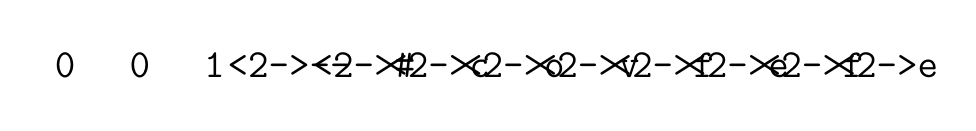
\begin{tikzpicture}[
			remember picture
		]
			\node[tmCell                ] (tmbandcell0) {};		

			\foreach \x  [count=\i] in {
				0,0,1,
				\only<2->{--},
				\only<2->{\#},
				\only<2->{c},
				\only<2->{o},
				\only<2->{v},
				\only<2->{f},
				\only<2->{e},
				\only<2->{f},
				\only<2->{e}
			} {
				\node[tmCell] at ($(tmbandcell0) + (\i*\cellSize,0) - (\cellSize,0)$) {\x};
			}
		\end{tikzpicture}
			

		\begin{tikzpicture}[overlay, remember picture]
			\only<1-2> {
				\handwrittenNoteBelow{tmbandcell0}{Eingabe}{+(2, -0.6)}
			}
		
			\only<1> {\tmDrawGrid{0}{3}}
			\only<2> {\tmDrawGrid{0}{12}}
			\only<3-> {
				\foreach \i in {1,...,5} {
					\node[tmCell, tmCellBlank] at ($(tmbandcell0) - (\i*\cellSize,0)$) {\only<4->{\tmBlankSym}};
					\node[tmCell, tmCellBlank] at ($(tmbandcell0) + (\i*\cellSize,0) + (11*\cellSize, 0)$) {\only<4->{\tmBlankSym}};
				}
				\tmDrawGrid{-5}{18}

				\handwrittenNoteBelow{tmbandcell0}{Speicher / Band}{+(2, -0.6)}
			}
			
			\only<5->{
				\node[tmHeadMarker, at=(tmbandcell0)] {};
				\handwrittenNoteAbove{tmbandcell0}{Kopf}{+(0.4, 0.4)}
			}
			
			\only<6->{
				\node[emorot, anchor=north, at=(tmbandcell0.south), yshift=-0.2em] {\Large $\Leftarrow, \Downarrow, \Rightarrow$};
			
			}
		\end{tikzpicture}
	\end{center}
\end{frame}
\def\turingAStateDef{
%%%%%% BEGIN-TM: turingI, B111-11B %%%%%
	\tmstate{firstMinus}{Suche Minus}  {}{}
	\tmstate{rightDigit}{Rechte Ziffer}{above right=of firstMinus}{}
	\tmstate{leftDigit} {Linke Ziffer} {below right=of firstMinus}{}
	\tmstate{cleanUp}   {Aufräumen}    {below right=of rightDigit}{}
	
	\tmstart{firstMinus}
	
	\tmtrans{firstMinus}{firstMinus}{\trans 11R }{loop below}{}
	\tmtrans{firstMinus.east}{rightDigit.west}{\trans --R}{above,sloped}{}
	
	\tmtrans{rightDigit}{rightDigit}{\trans --R}{loop above}{}
	\tmtrans{rightDigit}{leftDigit}{\trans 1-L}{bend right, below, left}{}
	\tmtrans{rightDigit.east}{cleanUp.west}{\trans BBL}{above, sloped}{}
	
	
	\tmtrans{leftDigit}{leftDigit}{\trans --L}{loop below}{}
	\tmtrans{leftDigit}{rightDigit}{\trans 1-R}{bend right, below, right}{}
	
	\tmtrans{cleanUp}{cleanUp}{\trans -BL}{loop below}{}
%%%%%% END-TM: turingI %%%%%
}

\newcommand{\tmADraw}[1]{
	\newcommand{\tmStateCurrent}{#1}

	\begin{center}
		\scalebox{0.9}{
			\tmDrawStates{\turingAStateDef}
		}
		
		\vspace{2em}
		
		\tmDrawBand
	\end{center}
	
	\begin{tikzpicture}[remember picture, overlay]
		\foreach \i in {1,...,10} {
			\node[tmCell, tmCellBlank] at ($(tmbandcell0) - (\i*\cellSize,0) + (\cellSize, 0)$) {\tmBlankSym};
			\node[tmCell, tmCellBlank] at ($(tmbandcell0) + (\i*\cellSize,0) + (\thetmBandCnt*\cellSize, 0)$) {\tmBlankSym};
		}
		
		\tmDrawGrid{-10}{20}
	\end{tikzpicture}
}


\newcommand{\tmACallback}[1]{\only<+>{\tmADraw{#1}}}
\tmSetup{A}{\turingAStateDef}

\begin{frame}{Subtraktion: $\ttunum{3} - \ttunum{2} =\ ?$}
	\tmExecute{A}{111-11B}{\tmACallback}
\end{frame}

\lstset{
	language=[LaTeX]{TeX},
	basicstyle=\small\sffamily,
	numbers=left,
	numberstyle=\tiny,
	commentstyle=\color{goetheblau},
	frame=tb,
	columns=fullflexible,
	showstringspaces=false,
	morekeywords={\tmstate, \tmstart, \tmtrans, \trans},
	escapechar={\$},
	xleftmargin=2em
}	

\newcommand{\unimportant}[1]{\textcolor{dunkelgrau!30}{#1}}
\newcommand{\tmkey}[1]{\textcolor{emorot}{#1}}
%\newcommand{\unimportant}[1]{\textcolor{sandgrau}{#1}}

\begin{frame}[fragile]{Turing Maschine in \LaTeX}

\begin{lstlisting}[]
% Zustaende {Schluessel}{Name}{Formatierung}
\tmstate{$\tmkey{firstMinus}$}{Suche Minus}{}{}
\tmstate{$\tmkey{rightDigit}$}{Rechte Ziffer}{$\unimportant{above right=of firstMinus}$}{}
\tmstate{$\tmkey{leftDigit}$}{Linke Ziffer}{$\unimportant{below right=of firstMinus}$}{}
\tmstate{$\tmkey{cleanUp}$}{Aufraeumen}{$\unimportant{below right=of rightDigit}$}{}

\tmstart{$\tmkey{firstMinus}$}

% Uebergaenge {VON}{NACH}{\trans XYZ: Wenn X gelesen, schreibe Y, bewege Kopf nach Z}
\tmtrans{$\tmkey{firstMinus}$}{$\tmkey{firstMinus}$}{\trans 11R }{$\unimportant{loop below}$}{}
\tmtrans{$\tmkey{firstMinus}$.east}{$\tmkey{rightDigit}$.west}{\trans --R}{$\unimportant{above,sloped}$}{}
\tmtrans{$\tmkey{rightDigit}$}{$\tmkey{rightDigit}$}{\trans --R}{$\unimportant{loop above}$}{}
\tmtrans{$\tmkey{rightDigit}$}{$\tmkey{leftDigit}$}{\trans 1-L}{$\unimportant{bend right, below, left}$}{}
\tmtrans{$\tmkey{rightDigit}$.east}{$\tmkey{cleanUp}$.west}{\trans BBL}{$\unimportant{above, sloped}$}{}
\tmtrans{$\tmkey{leftDigit}$}{$\tmkey{leftDigit}$}{\trans --L}{$\unimportant{loop below}$}{}
\tmtrans{$\tmkey{leftDigit}$}{$\tmkey{rightDigit}$}{\trans 1-R}{$\unimportant{bend right, below, right}$}{}
\tmtrans{$\tmkey{cleanUp}$}{$\tmkey{cleanUp}$}{\trans -BL}{$\unimportant{loop below}$}{}
\end{lstlisting}
\end{frame}

%
\makeatletter
\newcommand{\pausecounter}{\number\c@beamerpauses}
\newcommand{\thisslide}{\number\beamer@slideinframe}
\makeatother	


\def\disableSims{2}
\def\simConcepts{tm}
\newcommand{\simulateEdges}[2]{
	\only<-\intcalcDec{\disableSims}>{
		\begin{scope}[on background layer]
			\foreach \n/\p in {#1} {
				% default \p to {} if not defined (foreach will set it to \n)
				\ifthenelse{\equal{\n}{\p}}{\def\p{}}{}
				\path[simulates,\p] (#2) to node(#2-\n){} (\n);
			}
		\end{scope}
	}
}

\newcommand{\newconcept}[6]{
	% 1 key
	% 2 position rad
	% 3 position angle
	% 4 simulates (comma sep)
	% 5 name
	
	\only<\pausecounter->{
		% book keeping: add concept to list of concepts
		\xdef\simConcepts{\simConcepts,#1}
		
		\pgfmathsetmacro\posx{cos(#3)*#2}
		\pgfmathsetmacro\posy{sin(#3)*#2}
		
		\node[concept] (#1) at ($(tm)  + (\posx, \posy)$) {#5};
		
		\ifthenelse{\equal{#4}{}}{}{
			\simulateEdges{#4}{#1}
		}
	}
	
	\only<\pausecounter>{
		\node[minimum width=0.25\textwidth, anchor=west, at=(current page.west), xshift=1em] {
			\ifthenelse{\equal{\infopanelenable}{}}%
			{%
				\parbox{0.3\textwidth}{
					\IfFileExists{images/#1.pdf}{true-branch}{}
					\IfFileExists{images/#1.png}{\includegraphics[width=0.3\textwidth]{images/#1.png}\ }{}
					\IfFileExists{images/#1.jpg}{\includegraphics[width=0.3\textwidth]{images/#1.jpg}}{}%
				}
			}%
			{}
		};
	}

	\xdef\infopanelenable{}
}

\newcommand{\setInfoPanel}[1]{
	\def\infopanelenable{1}
	\only<\pausecounter>{
		\node[minimum width=0.25\textwidth, anchor=west, at=(current page.west), xshift=1em] {#1};
	}
}
\newcommand{\bsl}{{\tt \textbackslash}}


\begin{frame}[fragile]{}
	\xdef\simConcepts{tm}
	\begin{center}
		\begin{tikzpicture}[
			overlay, remember picture,
			conceptActive/.style={text=emorot, emorot, fill=emorot!10},
			concept/.style={dunkelgrau, text=black, draw, fill=sandgrau, rounded corners=0.4em, minimum height=1.6em, onslide={<\pausecounter> conceptActive},  align=center},
			simulatesActive/.style={emorot},
			simulates/.style={draw, ->, thick, opacity=0.5, onslide={<\pausecounter> simulatesActive}}
		]
		{
%			\renewcommand{\pause}{}
			
			\node[concept, at=(current page), xshift=4em] (tm) {Turing Machine};
			
			\pause
			\setInfoPanel{\parbox{0.26\textwidth}{
				\texttt{s\\/ZUSTAND-ALT:(.*)(.)@X(.*)\\/ZUSTAND-NEU:\bsl1@\bsl2Y\bsl3/}
			}}
			\newconcept{sed}{2}{45}{tm}{SED}{}
			
			\pause
			\setInfoPanel{				
				\parbox{0.28\textwidth}{
				\begin{center}
				
\includegraphics[width=0.15\textwidth]{images/python.png}
				\end{center}
			}}
			\newconcept{python}{4}{45}{}{Python}{}
			\only<\pausecounter->{			
				\path[simulates, bend left=40] (python) to (sed-tm);
			}
			
			\pause
			\only<\pausecounter->{			
				\path[simulates, bend right=40] (sed) to (sed-tm);
			}
			
			

			\pause
			\setInfoPanel{				
				\parbox{0.28\textwidth}{
				\begin{center}
				
\includegraphics[width=0.15\textwidth]{images/python.png}
				\end{center}
				\vspace{1em}	
				
				\fbox{\parbox{0.28\textwidth}{\small
				\textbf{if} state=="A":\\
				\phantom.\hspace{1em}\textbf{if} band.read()=="0":\\
				\phantom.\hspace{2em}band.write(1)\\
				\phantom.\hspace{2em}band.goLeft()\\
				\phantom.\hspace{2em}state = "B"\\
				\phantom.\hspace{1em}\textbf{elif} band.read()=="1":\\
				\phantom.\hspace{2em}\ldots\\
				\textbf{elif} state=="B":\\
				\phantom.\hspace{1em}\textbf{if} band.read()=="0":\\
				\phantom.\hspace{1em}\ldots
			}}}}
			\only<\pausecounter->{
				\simulateEdges{tm/bend right}{python}
			}
			
			
			\pause
			\setInfoPanel{				
				\parbox{0.32\textwidth}{
				\begin{center}
				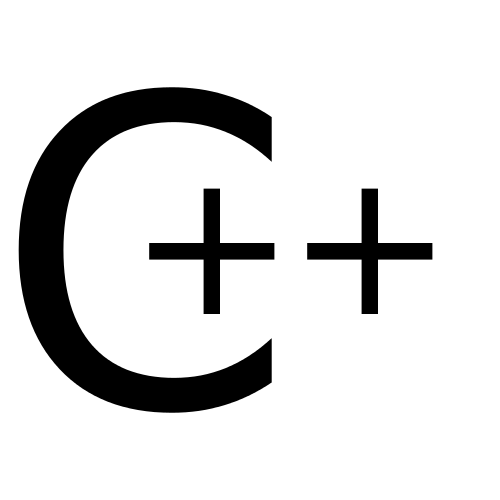
\includegraphics[width=0.15\textwidth]{images/cccc.png}
				\end{center}
				\vspace{1em}	
				
				\fbox{\parbox{0.32\textwidth}{\small
				\textbf{if} (state=='A') \{\\
				\phantom.\hspace{1em}\textbf{if}(band.read()=='0') \{\\
				\phantom.\hspace{2em}band.write(1)\\
				\phantom.\hspace{2em}band.goLeft()\\
				\phantom.\hspace{2em}state = "B"\\
				\phantom.\hspace{1em}\} \textbf{else if}(band.read()=='1') \{ \\
				\phantom.\hspace{2em}\ldots \}\\
				\} \textbf{else if}(state=="B") \{\\
				\phantom.\hspace{1em}\textbf{if}(band.read()=="0") \{\\
				\phantom.\hspace{1em}\ldots \}\}
			}}}}			
			\newconcept{cccc}{3}{20}{tm}{C/C++}{}
			
			\pause
			\newconcept{ctemp}{5}{20}{tm}{C++\\ templates}{}
		

			\pause
			\newconcept{javascript}{4}{3}{tm}{JavaScript}{}

			\pause
			\newconcept{excel}{2}{100}{tm}{Excel}{}

			\pause
			\newconcept{powerpoint}{3}{135}{tm}{Powerpoint}{}

			\pause
			\newconcept{email}{3}{155}{tm}{eMails}

			\pause
			\newconcept{gol}{3}{180}{tm}{Game of\\ Life}{}

			\pause
			\newconcept{rooz}{2.5}{210}{tm}{Rule 110}{}

			\pause
			\newconcept{htmlcss}{3.8}{220}{rooz}{CSS3}{}

			\pause
			\newconcept{dwarf}{2.5}{250}{tm}{Dwarf\\Fortress}{}

			\pause
			\newconcept{minecraft}{4}{240}{tm}{MineCraft}{}

			\pause
			\newconcept{factorio}{1.5}{280}{tm}{Factorio}{}

			\pause
			\newconcept{braid}{2.5}{290}{tm}{Braid}{}

			\pause
			\newconcept{littlebigplanet}{3.5}{280}{tm}{Little Big Planet}{}
		}
		
			\pause
			\only<\pausecounter->{
				\newconcept{ram}{4}{330}{}{Computer}{}
				\simulateEdges{ram}{tm}
			}

			\pause			
			\only<\pausecounter-\intcalcDec{\disableSims}>{
				
				\begin{scope}[on background layer]			
					\foreach \n in \simConcepts {
						\path[simulates,onslide={<\pausecounter> simulatesActive}] (ram) to (\n);			
					}
				\end{scope}
			}

			\pause
			\xdef\disableSims{\pausecounter}
			\only<\pausecounter->{
				\begin{scope}[on background layer]			
				\setInfoPanel{
\includegraphics[width=0.3\textwidth]{images/executeall.png}}

				\foreach \x in \simConcepts {
					\def\active{}
					\foreach \y in \simConcepts {
						\ifthenelse{\equal{1}{\active}}{
							\path[simulates,onslide={<\pausecounter> simulatesActive}, <->] (\x) to (\y);			

						}{}
						\ifthenelse{\equal\x\y}{\xdef\active{1}}{}
					}
					
					\path[simulates,onslide={<\pausecounter> simulatesActive}, loop left] (\x) to (\x);
				}
				\end{scope}
				
			}
		\end{tikzpicture}
	\end{center}
\end{frame}


\begin{frame}{Warum sind Turing Maschinen \emph{wirklich} nützlich?}
	\textcolor{goetheblau}{Was haben wir gesehen?} \\
	$\left.\text{\parbox{0.5\textwidth}{
		\begin{itemize}
			\item<2-> \textcolor{goetheblau}{sed} kann eine \textcolor{emorot}{Turing Maschine} ausführen
			\item<3-> Eine \textcolor{emorot}{Turing Maschine} kann \textcolor{goetheblau}{sed} ausführen
			\item<4->[$\Rightarrow$] Beide sind gleich mächtig!
		\end{itemize}
	}}
	\hspace{1em}
	\only<-4>{\right.}
	\only<5->{\right\}\hspace{1em} \textbf{Turing Vollständig}}
	$
\end{frame}

\begin{frame}{Was können Turing Maschinen \textbf{nicht}?}
	\begin{itemize}
		\item Eingabe/Ausgabe beschreiben
		\pause
		\item Schnell rechnen
		\pause
		
		\vspace{1em}

		\item Für ein \textcolor{goetheblau}{beliebiges} Programm $P$ entscheiden, 
		\begin{itemize}
			\item \ldots ob $P$ fertig wird
			\pause
			\item \ldots ob $P$ für eine feste Eingabe, eine feste Ausgabe berechnet
			\pause
			\item \ldots ob $P$ eine nicht triviale Eigenschaft erfüllt
		\end{itemize}

		\vspace{1em}

		\item 
		Bei \textcolor{goetheblau}{beliebigen} \textquotedblleft Domino-Steinen\textquotedblright{} berechnen,\\ ob man oben und unten diesselben Worte legen kann
	\end{itemize}
\end{frame}


\begin{frame}{Was ist nicht Turing-Vollständig?}
	\begin{itemize}
		\item 
			Reine Daten
			\begin{itemize}
				\item (Werte-)Tabellen
				\item HTML, XML
				\item Rechenschieber
			\end{itemize}
		
			\vspace{1em}
			
		\pause
		
		\item Endliche Automaten
			\begin{itemize}
				\item 
					Turing Maschine mit schreibgeschüztem Band
					
				\item
					Turing Maschine, die den Kopf nur nach rechts bewegen darf
					
				\item
					Reguläre Sprachen
					
				\item
					\texttt{sed} ohne Sprünge
			\end{itemize}
		
		\pause
		
		\item \ldots
	\end{itemize}
\end{frame}

\setbeamertemplate{footline}{} 
\goethccBgTitel
\begin{frame}{}
	\titlepage
	\begin{tikzpicture}[overlay]
	\node[anchor=south east, xshift=-0.08\textwidth, at=(current page.south east)] {
		\parbox{0.3\textwidth}{
		\begin{center}
			\scalebox{1.5}{\qrcode{http://nos17.manuel.jetzt}}
			
			\vspace{1em}
			
			\small\textcolor{goetheblau}{\url{http://nos.manuel.jetzt}}
		\end{center}
	}};
	\end{tikzpicture}
\end{frame}




\end{document}

